%!TEX root = Thesis.tex
\chapter{Foundations and Requirements Analysis}

\section{Terminology}
The fundamental terms used in this thesis are described below for better understanding of the presented research work.
\subsection {Frontend and Criteria}
In computer science, the front end is responsible for collecting input in various forms from the user and processing it to conform to a specification the backend can use. The frontend is an interface between the user and the backend\cite{wiki:xxx} and the separation of software systems into front and back ends simplifies development and separates maintenance. Therefore need to be distinguished what are the main requirements to a generic frontend for exploring sensed data.
\begin{itemize}
\item Loosely-coupling
\item Fine-grained structure
\item Multy-user capability
\item Cross-platforming
\item Adaptivity
\end{itemize}

\subsubsection {Web Portal}
Such a system, that generates requested information dynamically, displays that
information in a useful manner in Web, maintains control over the created/saved files, automatically updates
the information, and supports a distributed environment\cite{rezayat2000enterprise}.
A web portal is most often specially-designed Web page at a website which brings information together from diverse sources in a uniform way. Usually, each information source gets its dedicated area on the page for displaying information (a portlet); often, the user can configure which ones to display.Portals provide a way for enterprises and organizations to provide a consistent look and feel with access control and procedures for multiple applications and databases, which otherwise would have been different web entities at various URLs. The features available may be restricted by whether access is by an authorized and authenticated user (employee,member) or an anonymous site visitor\cite{wiki:portal}.

\subsubsection {Mashup}
The mashup application is a composite Web 2.0 application that aggregates and
integrates heterogeneous web resources offered in a form of available Web APIs and
sources for creating a new service. Mashups differ from traditional component-based
applications in providing more situational character of these applications\cite{yu2008understanding}.
In general there distinguish the following three types of mashups\cite{peenikal2009mashups}. 
Customer mashups are aimed at the combination and reformation data from various
public sources according to users’ needs. Data mashups aggregate similar types of
resources from diverse sources into a new single data representation. And business,
or enterprise, mashups define composite applications that are focused on solving
heterogeneous business problems by supporting collaborative activities\cite{hoyer2008enterprise}.
Concerning architectural styles of mashup applications,
 server-side and clientside mashups are distinguished. In the server-side mashups a content aggregation
is realized on a server. The server plays a role of a proxy between the
mashup application and other web sites that involved in this application. The
opposite client-side mashups aggregate content on a client, typically, at a client’s
web browser\cite{ort2007mashup}.
Earlier, composite web applications covered the integration at the low application
layers, such as the traditional data and business logic layers. However, mashups with
their intention to reuse pieces of user interfaces (UIs) from different web resources
increase the necessity of the UI integration, and the composition at the presentation
layer\cite{daniel2007understanding}. Several research approaches refer to the problem of the component-
based development of web applications at the presentation layer\cite{pietschmann2010application}.
\subsection {Sensor Data Streams}

\section{Web-based Framework Analysis}
 \begin{itemize}
\item \textbf{Bootstrap}
\newline
Bootstrap is the most popular and widely used framework, nowadays. It’s a beautiful, intuitive and powerful web design kit for creating cross browser, consistent and good looking interfaces. It offers many of the popular UI components with a plain-yet-elegant style, a grid system and JavaScript plugins for common scenarios.

It is built with LESS and consists of four main parts:
Scaffolding – global styles, responsive 12-column grids and layouts. Bear in mind that Bootstrap doesn’t include responsive features by default. If design needs to be responsive this functionality have to be done manually.
Base CSS – this includes fundamental HTML elements like tables, forms, buttons, and images, styled and enhanced with extensible classes.
Components – collection of reusable components like dropdowns, button groups, navigation controls (tabs, pills, lists, breadcrumbs, pagination), thumbnails, progress bars, media objects, and more.
JavaScript – jQuery plugins which bring the above components to life, plus transitions, modals, tool tips, popovers, scrollspy (for automatically updating nav targets based on scroll position), carousel, typeahead (a fast and fully-featured autocomplete library), affix navigation, and more.
\item \textbf{Foundation}
\newline
Foundation is a powerful, feature-rich, responsive front-end framework. With Foundation user can quickly prototype and build websites or apps that work on any kind of device, with tons of included layout constructs, elements and best practices. It’s built with mobile first in mind, utilitizes semantic features, and uses Zepto instead of jQuery in order to brings better user experience and faster performance.

Foundation has a 12-column flexible, nestable grid powerful enough to create rapidly multi-device layouts. In terms of features it provides many. There are styles for typography, buttons, forms, and various navigation controls. Many useful CSS components are provided like panels, pricing tables, progress bars, tables, thumbnails, and flex video that can scale properly your video on any device. And, of course, JavaScript plugins including dropdowns, joyride (a simple and easy website tour), magellan ( a sticky navigation that indicates where is the user on the page), orbit (a responsive image slider with touch support), reveal (for creating modal dialogs or pop-up windows),  sections (a powerful replacement for traditional accordions and tabs), and tooltips.
\item \textbf{GroundworkCSS}
\newline
GroundworkCSS is a new, fresh addition to the front-end frameworks family. It’s a fully responsive HTML5, CSS and JavaScript toolkit built with the power of Sass and Compass which gives the ability to rapidly prototype and build websites and apps that work on virtually any device.

It offers an extremely flexible, nestable, fraction-based, fluid grid system that makes creating any layout possible. GroundworkCSS has some really expressive features like tablets and mobile grids which maintain the grid column structure instead of collapsing the grid columns into individual rows when the viewport is below 768 or 480 pixels wide. Another cool feature is a jQuery ResponsiveText plugin which allows to have dynamically sized text that adapts to the width of the viewport: extremely useful for scalable headlines and building responsive tables.
The framework includes a rich set of UI components like tabs, responsive data tables, buttons, forms, responsive navigation controls, tiles (a beautiful alternative to radio buttons and other boring standard form elements), tooltips, modals, Cycle2(a powerful, responsive content slider), and many more useful elements and helpers. It also offers a nice set of vector social icons and a full suite of pictographic icons included in FontAwesome.
To see the framework in action user can use the resizer at the top center of the browser window. This way user can test the responsiveness of the components against different sizes and viewports while exploring the framework’s features.
GroundworkCSS is very well documented with many examples, and to get user started quickly the framework also provides several responsive templates. The only thing as a weakness is the missing of a way to customize download.

\item \textbf{Gumby}            
\newline
Gumby is simple, flexible, and robust front-end framework built with Sass and Compass.

Its fluid-fixed layout self-optimizes the content for desktop and mobile resolutions. It support multiple types of grids, including nested ones, with different column variations. Gumby has two PSD templates that get user started designing on 12 and 16 column grid systems.
The framework offers feature-rich UI Kit which includes buttons, forms, mobile navigation, tabs, skip links, toggles and switches, drawers, responsive images, retina images, and more. Following the latest design trends the UI elements have Metro style flat design but can use Pretty style with gradient design too, or to mix up both styles. An awesome set of responsive, resolution independent Entypo icons, is completely integrated into the Gumby Framework. Gumby has also a very good customizer with color pickers which helps to build your custom download with ease.
\item \textbf{Kube}
\newline
Lastly, if user need a solid, yet simple base without needless complexity and extras, for your new project, Kube can be the right choice. Kube is a minimal, responsive and adaptive framework with no imposed styling which gives to user the freedom to create. It offers basic styles for grids, forms, typography, tables, buttons, navigation, and other stuff like links or images.

The framework contains one compact CSS file for building responsive layouts with ease and two JS files for implementing tabs and buttons in your designs. If user is looking for maximum flexibility and customization, user can download developer version which includes LESS files, with variables, mixins and modules.
\end{itemize}

\begin{figure}[!ht]
\centering
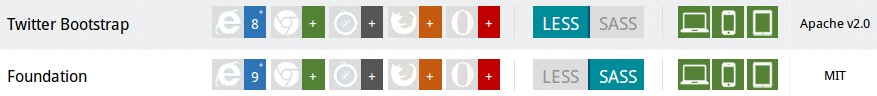
\includegraphics[scale=0.7]{images/Bootstrap&Foundation.png}
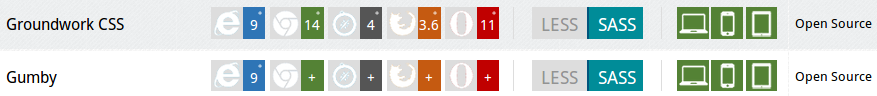
\includegraphics[scale=0.7]{images/Groundwork&Gumby.png} 

\includegraphics[scale=0.7]{images/Kube.png}  
\caption[Framework Comparison]{Framework Comparison\footnote{\url{http://usablica.github.io/front-end-frameworks/compare.html}}}
\label{img:Bootstrap&Foundation.png}
\label{img:Groundwork&Gumby.png}   
\label{img:Kube.png}                          
\end{figure}

\section{Prototype Requirements}
Like most modern applications, each of these is structured into three layers: presentation, 
application (also called the business-logic layer), and data.
\begin{enumerate}
\item the granularity of the functions that the component applications provide is generally well
suited for high-level integration (for example, we can tell an application to begin monitoring
machine xyz without considering how this activity will affect data in the integrated application’s database)
\item it’s more stable because the component application is aware of the integration (it exposes
the API) and will attempt to stabilize the interface across versions
\end{enumerate}

\section{Summary}